Two families: symmetric cryptosystems use the same key for encryption and decryption. They rely on the principles from classical systems: substitution, permutation, and transposition. The reversing operation is dependent on the key.
Asymmetric cryptosystems, on the other hand, use a pair of mathematically related keys—one for encryption (public key) and another for decryption (private key)—relying on complex mathematical problems for security.

\subsection{Block Ciphers}
\begin{defn}
A \textbf{block cipher} is a deterministic cryptographic algorithm that operates on fixed-size blocks of data, typically \( n \) bits, using a symmetric key to perform encryption or decryption. It transforms a plaintext block of size \( n \) bits into a ciphertext block of the same size through a series of reversible, structured operations, and vice versa.

\end{defn}
\begin{figure}[h!]
    \centering
    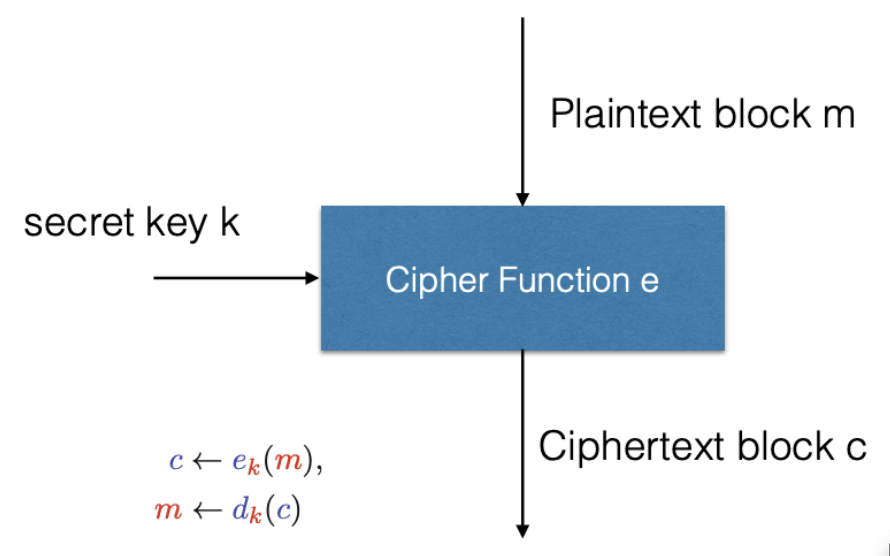
\includegraphics[width=0.5\textwidth]{img/blockcipher.png}
    \caption{Block Cipher}
    \label{fig:block_cipher}
\end{figure}

where
\begin{itemize}
    \item $m \in \{0,1\}^n$ is the plaintext block,
    \item $k \in K$ is the secret key, chosen from key space K,
    \item $e$ is the encryption function,
    \item $d$ is the decryption function,
    \item $c \in \{0,1\}^b$ is the ciphertext block.
\end{itemize}

NOTE: Block ciphers are not proper encryption schemes. You need to combine them with modes of operation! Otherwise your system will not be secure.

\subsubsection{Properties of Block Ciphers}
\begin{enumerate}
    \item Input data block: Plaintext is divided into equal-sized blocks.
    \item Encryption/Decryption: Each block undergoes multiple transformations (substitution, permutation, and mixing) to produce ciphertext.
    \item Key: A symmetric key is applied in multiple \emph{rounds} to ensure security.
    \item Padding: If the last block of plaintext is smaller than the block size, padding is added.
    \item Modes of operation: Block ciphers work with data larger than one block by using modes like:
    \begin{itemize}
        \item ECB (Electronic Codebook)
        \item CBC (Cipher Block Chaining)
        \item GCM (Galois/Counter Mode)
    \end{itemize}
\end{enumerate}
Block ciphers are typically \emph{64 bits} (in DES), \emph{128 bits} (in AES) or more (in modern ciphers). They should act like a \emph{pseudorandom permutation} (PRP).

\begin{defn}
A \textbf{pseudorandom permutation} (PRP) is a function that defines a bijective (one-to-one and onto) mapping between input and output spaces, such that it is computationally indistinguishable from a truly random permutation when the key is unknown. 
\end{defn}

In order to limit the advantage of the adversary, the key space is kept very large (e.g. $Adv \ 1/|K|$). A block cipher is a \emph{building block} for designing a cipher (a PRP). A block cipher with a \emph{Mode of Operation} is a cipher. The goal is to design an IND-CCA secure cipher.

\subsubsection{Design}
DES and AES are iterated block ciphers. They \emph{repeat a simple round function}. The round $r$ can be fixed or variable. The more rounds, the higher the security of the cipher.
\begin{itemize}
    \item In each round, a round key, derived from the key $k$, is used (by key scheduling algorithm) to process a block
    \item The round function should be \emph{invertible}; for decryption the round keys are used in reverse order
    \item In DES: the round is invertible but not the round function
    \item In AES: both the round and the round function are invertible
\end{itemize}

\begin{defn}
    The \textbf{confusion-diffusion} paradigm is a fundamental design principle for secure cryptographic systems, particularly block ciphers.
    \begin{itemize}
        \item \textbf{Confusion:} Confusion ensures that the relationship between the key and the ciphertext is highly complex, making it difficult for an attacker to infer the key, even if they have access to multiple plaintext-ciphertext pairs. Split the block into smaller blocks and apply a
        substitution on each block.
        \item \textbf{Diffusion:} Diffusion ensures that the influence of a single bit of plaintext (or key) spreads widely over the ciphertext, so that changes in input affect many output bits.  Mix permutations so that local change can effect the
        whole block.
    \end{itemize}
\end{defn} \label{def:confusion_diffusion}

\begin{defn}
    A \textbf{substitution-permutation network} (SPN) is a design model for block ciphers. It consists of a series of linked operations, including substitution, permutation, and key mixing. It is a direct implementation of defintion \ref{def:confusion_diffusion}. 
\end{defn}
See figure \ref{fig:spn} for a diagram of an SPN.
\Comment{watch video on this for extra notes}

\subsubsection{The Avalanche Effect}
A small change in the input must affect every bit of the output. This is called the \emph{avalanche effect}. It is a desirable property of block ciphers.
\begin{enumerate}
    \item The S-boxes (substitution box) are designed such that 1 bit effects at least 2 bits in the output of the boxes
    \item The mixing permutations are designed
\end{enumerate}

In principle, you need at least 7 rounds for a good diffusion. This is mathematically shown (outside of context for this course). Too few rounds (e.g. 1 or 2) will not provide security. The rounds can easily be reverted. 

\subsection{Feistel Ciphers}
\begin{defn}
A \textbf{Feistel cipher} is a symmetric structure used to construct block ciphers, including DES. It splits the plaintext block into two halves and performs a series of rounds of processing on the halves. Each round applies a function $F$ to one half and then combines it with the other half using a reversible operation, typically XOR.
\end{defn}

\begin{figure}[h!]
    \centering
    \begin{minipage}[t]{0.35\textwidth}
        \centering
        \vspace{0pt} % Ensure top alignment
        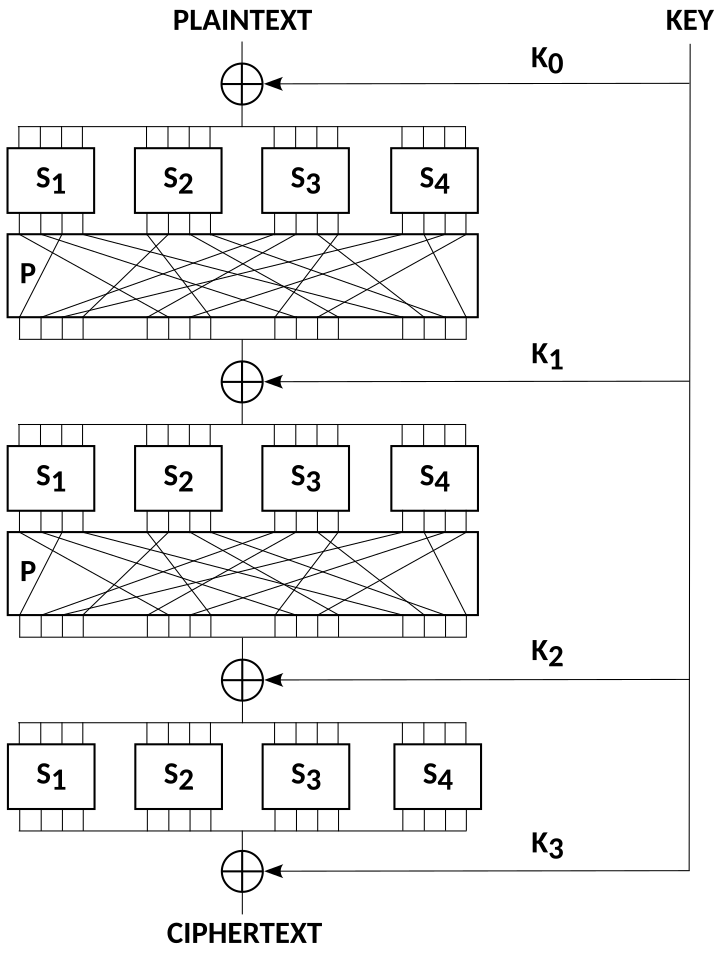
\includegraphics[width=\textwidth]{img/spn.png}
        \caption{A sketch of a substitution–permutation network with 3 rounds, encrypting a plaintext block of 16 bits into a ciphertext block of 16 bits. The S-boxes are the Si, the P-boxes are the same $P$, and the round keys are the $K_i$.}
        \label{fig:spn}
    \end{minipage}
    \hfill
    \begin{minipage}[t]{0.45\textwidth}
        \vspace{0pt} % Ensure top alignment
        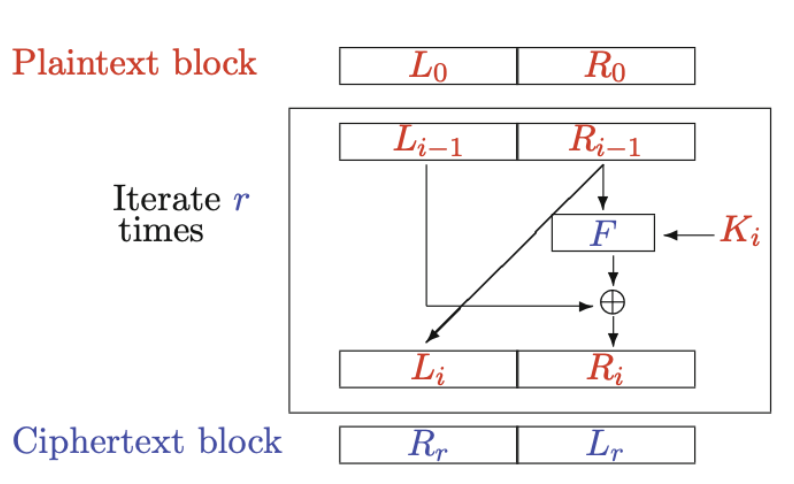
\includegraphics[width=\textwidth]{img/feistel.png}
        \caption{Basic operation of a Feistel cipher}
    \end{minipage}
\end{figure}

In a Feistel cipher, the round function is \emph{invertible}. It is different from an SPN, as that one is based on a non-invertible component. We can choose any function $F$ and still the round is invertible.
The same hardware/software can be used for encryption and decryption (just use the keys in reverse order). The security of the cipher depends on: the round keys, the number of rounds, and the function $F$.

\subsubsection{Encryption}
Given a plaintext block \( P \), a Feistel cipher processes it as follows:

\begin{enumerate}
    \item Initial split: Divide \( P \) into two equal-sized halves:
    \[
    P = (L_0, R_0)
    \]
    where \( L_0 \) and \( R_0 \) are the left and right halves, respectively.

    \item Rounds of encryption: For each round \( i \) (1 to \( n \)), compute:
    \[
    L_i = R_{i-1}
    \]
    \[
    R_i = L_{i-1} \oplus F(R_{i-1}, K_i)
    \]
    where:
    \begin{itemize}
        \item \( F \) is the round function (a non-linear function).
        \item \( K_i \) is the round key for round \( i \), derived from the main key.
    \end{itemize}

    \item Final Swap (Optional): After \( n \) rounds, the ciphertext \( C \) is obtained as:
    \[
    C = (R_n, L_n)
    \]
    (Note: The final swap is optional and does not affect decryption.)
\end{enumerate}

\subsubsection{Decryption}

The Feistel structure makes decryption straightforward because it is inherently reversible. Using the ciphertext \( C = (R_n, L_n) \):

\begin{enumerate}
    \item Initialize \( R_n \) and \( L_n \) as inputs.
    \item For each round \( i \) (in reverse order, from \( n \) to 1):
    \[
    R_{i-1} = L_i
    \]
    \[
    L_{i-1} = R_i \oplus F(L_i, K_i)
    \]
    \item Combine \( L_0 \) and \( R_0 \) to recover the original plaintext.
\end{enumerate}

The same function \( F \) and subkeys \( K_i \) are used in both encryption and decryption, but the subkeys are applied in reverse order during decryption.

\subsection{Data Encryption Standard (DES)}
DES is one of the earliest widely-used block ciphers. Not used anymore. But, still in ATMs (3DES). Key features are:

\begin{itemize}
    \item Block size: 64 bits
    \item Key length: 56 bits (with 8 parity bits)
    \item Number of rounds: 16
    \item 16 round keys, 48 bits each
    \item Structure: Feistel cipher
\end{itemize}

In the Feistel structure, each round splits the input into two halves: One half is directly passed to the next round. The other half is transformed using a combination of substitution, permutation, and the round key, then XORed with the other half.

\begin{figure}[h!]
    \centering
    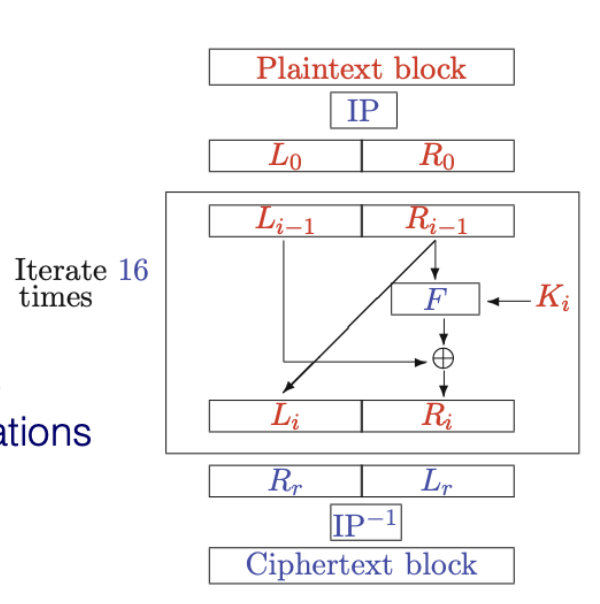
\includegraphics[width=0.35\textwidth]{img/des.png}
    \caption{DES as a Feistel structure}
    \label{fig:des}
\end{figure}

Operations:
\begin{itemize}
    \item 64 bits of plaintext block
    \item Perform an initial permutation (IP)
    \item Split the block into a left and right part
    \item Perform 16 rounds of \emph{identical operations}
    \item Join the half blocks together
    \item Perform a final reverse permutation (IP$^{-1}$)
\end{itemize}

\textbf{Decryption is identical to encryption: rounds keys in reversed order!} One algorithm is used for encryption and decryption. The same hardware can also be used for both.
DES is based on a Feistel structure. All that is needed to specify DES is a round function, a key schedule, and any additional processing (initial and final permutation).

\subsubsection{Function \texorpdfstring{$F$}{F}}
\begin{itemize}
    \item Expansion permutation: the right half 32 bits is expanded to 48 bits
    \item Round key addition: XOR with the round key 
    \item Splitting: 48 bits are split into 8 lots of 6-bit values
    \item S-boxes: non-linear part, output is 32 bits (8 lots of 4-bit values)
    \item P-box: Combine the previous lots to form a 32-bit value and apply permutation to form the output of $F$
\end{itemize}


\begin{figure}[h!]
    \centering
    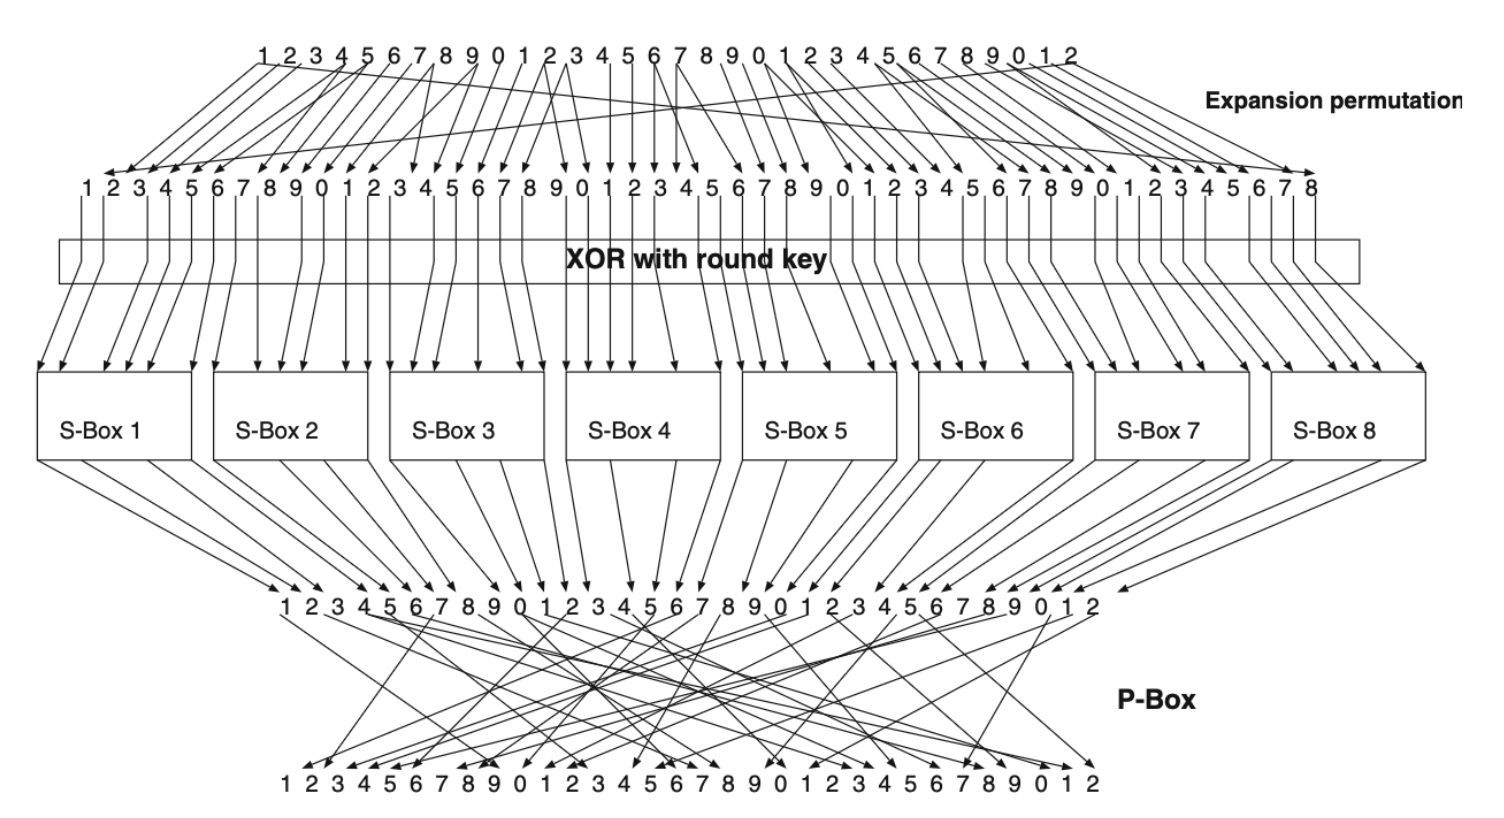
\includegraphics[width=0.5\textwidth]{img/desF.png}
    \caption{Structure of DES function \( F \)}
    \label{fig:f}
\end{figure}

\subsubsection{S-boxes}
In the \textbf{S-box} in the function $F$, the 48-bit result is divided into 8 groups of 6 bits. Each group of 6 bits is passed through a corresponding S-box, reducing it to 4 bits. \\

The S-box takes a 6-bit input and produces a 4-bit output. The 6-bit input is divided as follows:
\begin{itemize}
    \item The \textbf{first and last bits} (bits 1 and 6) are used to determine the \textbf{row number}.
    \item The \textbf{middle 4 bits} (bits 2, 3, 4, and 5) are used to determine the \textbf{column number}.
\end{itemize}

The row and column values are used to look up the corresponding 4-bit value in the S-box table (see lecture slides). DES uses 8 S-boxes, denoted \( S_1, S_2, \dots, S_8 \). Each S-box takes a 6-bit input and produces a 4-bit output. Together, the 8 S-boxes process the 48-bit input and reduce it to a 32-bit output.
The S-boxes are important for the following reasons:
\begin{itemize}
    \item Non-linearity: the S-box is the only non-linear component of the F-function, which makes DES resistant to linear and differential cryptanalysis.
    \item Confusion: S-boxes obscure the relationship between the plaintext, ciphertext, and the key.
    \item Compression: S-boxes reduce the 48-bit input to 32 bits, balancing the size for further processing.
\end{itemize}

\subsubsection{Permutations and P-box}
The \textbf{initial an final permutatations} are straight P-boxes that are inverses of each other. These permutations do not add cryptographic strength but are part of the standard DES algorithm.
\begin{itemize}
    \item The IP rearranges the 64-bit plaintext input bits into a new order. It is applied only once at the very beginning of the DES encryption process
    \item  The IP$^{-1}$ reverses the effect of the IP. It rearranges the bits of the 64-bit block back to their original positions
    \item IP and IP$^{-1}$ tables to specify how the input bits rearranged by index (see lecture slides for the tables)
\end{itemize}

The \textbf{expansion permutation} in the F-function of DES is a crucial step within each round of the encryption process. It is used to expand the 32-bit half-block input into 48 bits.
\begin{itemize}
    \item Bit duplication
    \item Introduce non-linearity: duplicating and rearranging bits makes it harder for an attacker to analyze relationships between plaintext, ciphertext, and the key.
    \item Kex mixing: XOR with the 48-bit round key
    \item Table in lecture slides
\end{itemize}

The \textbf{P-box} rearranges the bits of a given input in a specified order. The purpose of this permutation is to spread the influence of each bit across the output to enhance security by increasing diffusion. The P-box is used after the S-box substitution stage within the Feistel structure of DES. The S-box reduces the input to 32 bits, and the P-box permutes these 32 bits to prepare them for the next round of processing.

\subsubsection{Key Scheduling}
The \textbf{Key scheduling} process in DES generates 16 \textbf{subkeys} (48 bits each) from the original \textbf{64-bit key}. These subkeys are used in the 16 Feistel rounds of DES encryption. The key scheduling process consists of the following main steps:
\begin{enumerate}
    \item Initial 64-bit key is reduced to 56 bits by removing parity bits using the \textbf{PC-1} table.
    \item The 56-bit key is split into two 28-bit halves: \( C_0 \) and \( D_0 \).
    \item For each of the 16 rounds, both halves undergo \textbf{left circular shifts} (1 or 2 bits depending on the round).
            \[ C_i \leftarrow C_{i-1} \lll p_i \]
            \[ D_i \leftarrow D_{i-1} \lll p_i \]

        where $p_i$ is the cyclic shift.
    \item Combine the two halves. The \textbf{PC-2} table compresses the 56-bit key (combined \( C_i \) and \( D_i \)) into a 48-bit subkey.
    \item This process is repeated 16 times to generate 16 unique subkeys.
\end{enumerate}

\begin{figure}[h!]
    \centering
    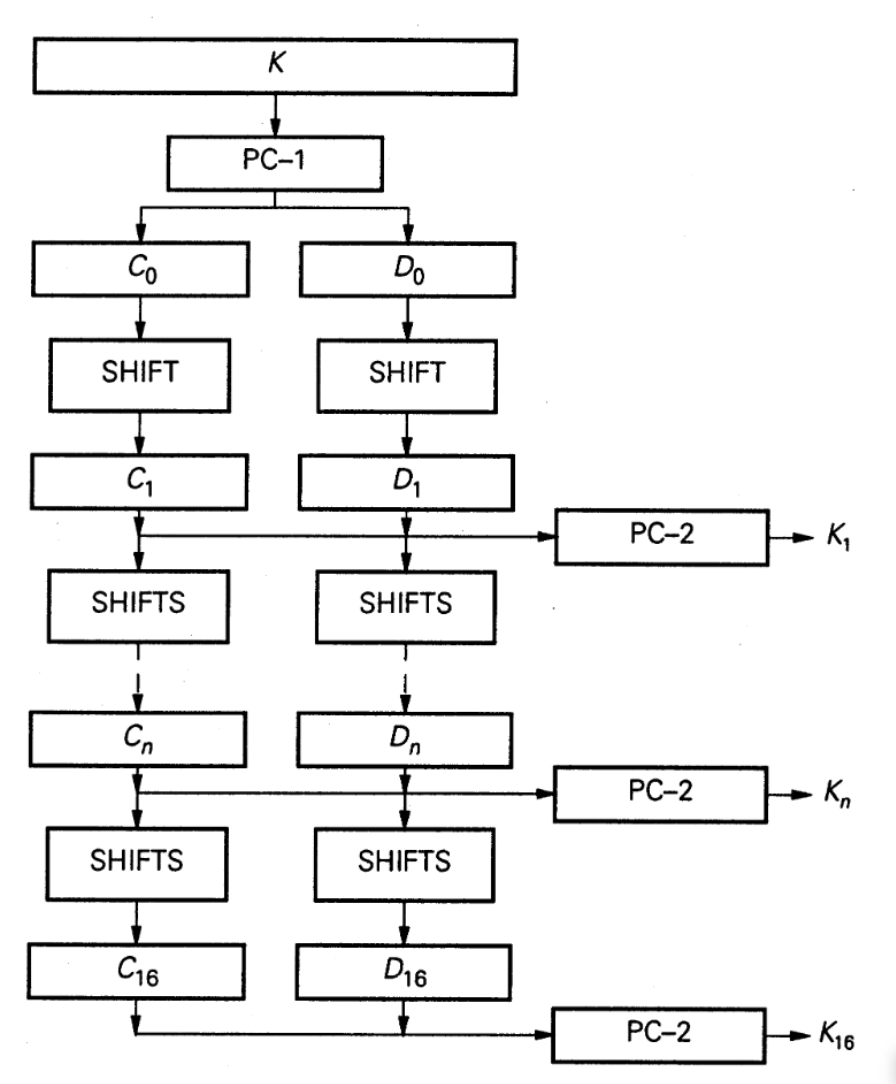
\includegraphics[width=0.3\textwidth]{img/DESkey.png}
    \caption{DES key scheduling}
    \label{fig:key}
\end{figure}

The key schedule ensures that even a small change in the original key produces completely different subkeys.




\subsubsection{Security of DES}
1, 2, and 3-round DES is not secure. DES in general is not secure! Can be cracked with exhaustive search. But: costs a lot of time or memory. Time-space tradeoff: with more memory, a few minutes is sufficient. The 56-bit key length is vulnerable to brute-force attacks (exhaustive search). Modern computational power can crack DES in hours. 
However, to crack DES you need mathematical, puzzle-solving skills and \emph{luck}. \\

The key length is the weakest point in DES. Then can't we just encrypt twice, using two keys? The key space would become $2^{n\cdot k} = 2^{112}$ with $n = 2, k = 56$. Unfortunately, this is not true. The key space remains $2^{56}$:

When trying to improve the security of a block cipher, a tempting idea is to encrypt the data several times using multiple keys. One might think this doubles or even n-tuples the security of the multiple-encryption scheme, depending on the number of times the data is encrypted, because an exhaustive search on all possible combinations of keys (simple brute force) would take $2^{n\cdot k}$ attempts if the data is encrypted with $k$-bit keys $n$ times. \\

\begin{figure}[h!]
\centering
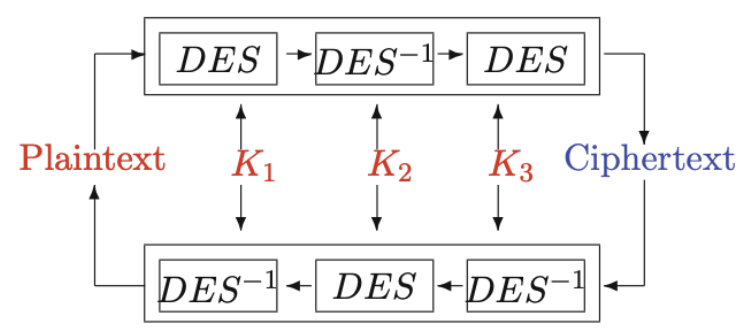
\includegraphics[width=0.4\textwidth]{img/3DES.png}
\caption{Triple DES}
\end{figure}

The \textbf{meet-in-the-middle attack} (MITM) is a generic attack that weakens the security benefits of using multiple encryptions by storing intermediate values from the encryptions or decryptions and using those to improve the time required to brute force the decryption keys. 
The attack attempts to find the keys by using both the range (ciphertext) and domain (plaintext) of the composition of several functions (or block ciphers) such that the forward mapping through the first functions is the same as the backward mapping (inverse image) through the last functions, quite literally meeting in the middle of the composed function. For example, although Double DES encrypts the data with two different 56-bit keys, Double DES can be broken with $2^{57}$ encryption and decryption operations.
The MITM attack is the primary reason why 2DES is not used, and 3DES can be brute-forced by an attacker with $2^{56}$ space and $2^{112}$ operations.


\subsubsection{Cryptanalysis of Block Ciphers}
Can be done with:
\begin{itemize}
    \item Exhaustive search
    \item Pre-computed intermediate values
    \item Divide and conquer
\end{itemize}

A block cipher should be resistant against differential and linear cryptanalysis. \Comment{explain what this is?}

\subsection{Advanced Encryption Standard (AES)}
AES replaced DES in the 1990s. Public design. AES is not a Feistel cipher, but a SPN. It is based on the Rijndael algorithm. Key features are:
\begin{itemize}
    \item Each round has a key addition phase, a substitution phase (non-linear, confusion), and a permutation phase (for diffusion, avalanche effect)
    \item AES is built on a mathematical foundation (finite fields $\mathbb{F}_{2^8}, \mathbb{F}_2$)
    \item Encryption and decryption are distinct operations (do not rely \emph{solely} on reverse ordering of the keys)
    \item Supports multiple key lengths: 128, 192, and 256 bits (and thus also blocks of these sizes)
\end{itemize}

\subsubsection{Finite Fields and Arithmatic in AES}
Elements of $\mathbb{F}_{2^8}$ are stored as bit vectors (or bytes) representing \textbf{binary polynomials}. From the hexadecimal representation of a byte, we can derive the polynomial representation. For example, the byte \texttt{0x57} is represented by the polynomial $x^6 + x^4 + x^2 + x + 1$. The polynomial representation is used for arithmetic operations in AES.

\[ \texttt{0x57} = 5 \cdot 16 + 7 = 87 \] in decimal. The bit representation in binary is given by concatenating the bit representation of 5 and 7:

\[\texttt{0101 0111}\]

The bit pattern then corresponds to the binary polynomial, using the indexes where the bits are set to 1 as the exponents of the polynomial:

\[ x^6 + x^4 + x^2 + x + 1\] 

Arithmethic in the finite field $\mathbb{F}_{2^8}$ is a cornerstone of the AES algorithm. It is a Galois field with $2^8 = 256$ elements. \\

\textbf{Field Construction}
\begin{itemize}
    \item \(\mathbb{F}_{2^8}\) is constructed as a polynomial field over \(\mathbb{F}_2\) (the field with two elements, \(0\) and \(1\)).
    \item Elements of \(\mathbb{F}_{2^8}\) are represented as polynomials of degree at most 7 with coefficients in \(\mathbb{F}_2\). For example:
    \[
    a(x) = a_7x^7 + a_6x^6 + \cdots + a_1x + a_0, \quad a_i \in \{0, 1\}.
    \]
    \item Addition and multiplication of elements are defined modulo an irreducible polynomial \(m(x)\) of degree 8 over \(\mathbb{F}_2\). In AES, the chosen irreducible polynomial is:
    \[
    m(x) = x^8 + x^4 + x^3 + x + 1.
    \]
\end{itemize}

\textbf{Addition}
\begin{itemize}
    \item Addition in \(\mathbb{F}_{2^8}\) corresponds to bitwise XOR of the coefficients of the two polynomials.
    \item Example:
    \[
    (a_7x^7 + a_6x^6 + \cdots + a_0) + (b_7x^7 + b_6x^6 + \cdots + b_0)
    = (a_7 \oplus b_7)x^7 + \cdots + (a_0 \oplus b_0).
    \]
\end{itemize}

\textbf{Multiplication}
\begin{enumerate}
    \item \textbf{Polynomial Multiplication}:
    \begin{itemize}
        \item Multiply two polynomials \(a(x)\) and \(b(x)\) normally, treating them as polynomials over \(\mathbb{F}_2\).
        \item Example:
        \[
        a(x) = x^2 + 1, \quad b(x) = x^3 + x
        \]
        \[
        a(x) \cdot b(x) = (x^2 + 1)(x^3 + x) = x^5 + x^3 + x^3 + x = x^5 + x.
        \]
    \end{itemize}
    \item \textbf{Modulo Reduction}:
    \begin{itemize}
        \item Reduce the result modulo the irreducible polynomial \(m(x)\).
        \item For example, if \(a(x) \cdot b(x) = x^9 + x^5\), reduce it modulo \(x^8 + x^4 + x^3 + x + 1\):
        \[
        x^9 = x \cdot x^8 \equiv x(x^4 + x^3 + x + 1) \mod m(x).
        \]
    \end{itemize}
    \item The final result after reduction is the product in \(\mathbb{F}_{2^8}\).
\end{enumerate}

\textbf{Inversion}
\begin{itemize}
    \item Inversion (finding the multiplicative inverse) is critical in the AES S-box.
    \item The inverse of an element \(a(x)\) in \(\mathbb{F}_{2^8}\) is the unique element \(b(x)\) such that:
    \[
    a(x) \cdot b(x) \equiv 1 \mod m(x).
    \]
    \item This is typically computed using the Extended Euclidean Algorithm.
\end{itemize}

\subsubsection{State Matrix}
AES organizes the input plaintext (or ciphertext) as a 4x4 matrix of bytes called the state. Each entry in the matrix is one byte (8 bits), and the matrix evolves through each round of AES encryption or decryption. Each round key is held by a 4x4 matrix.

\[ S = \begin{pmatrix}
    s_{0,0} & s_{0,1} & s_{0,2} & s_{0,3} \\
    s_{1,0} & s_{1,1} & s_{1,2} & s_{1,3} \\
    s_{2,0} & s_{2,1} & s_{2,2} & s_{2,3} \\
    s_{3,0} & s_{3,1} & s_{3,2} & s_{3,3} \\
\end{pmatrix},
K_i = \begin{pmatrix}
    k_{0,0} & k_{0,1} & k_{0,2} & k_{0,3} \\
    k_{1,0} & k_{1,1} & k_{1,2} & k_{1,3} \\
    k_{2,0} & k_{2,1} & k_{2,2} & k_{2,3} \\
    k_{3,0} & k_{3,1} & k_{3,2} & k_{3,3} \\
\end{pmatrix} \] \\

\textbf{Mapping Input Plaintext to the State Matrix}
\begin{itemize}
    \item AES operates on 128-bit blocks (16 bytes) at a time.
    \item The 128-bit plaintext block is split into 16 bytes and arranged column-by-column into the state matrix.
\end{itemize}

For a plaintext block:
\[
P = [\text{byte}_0, \text{byte}_1, \dots, \text{byte}_{15}],
\]
the state matrix is represented as:
\[
S = 
\begin{pmatrix}
\text{byte}_0 & \text{byte}_4 & \text{byte}_8  & \text{byte}_{12} \\
\text{byte}_1 & \text{byte}_5 & \text{byte}_9  & \text{byte}_{13} \\
\text{byte}_2 & \text{byte}_6 & \text{byte}_{10} & \text{byte}_{14} \\
\text{byte}_3 & \text{byte}_7 & \text{byte}_{11} & \text{byte}_{15}
\end{pmatrix}.
\]

\subsubsection{AES Operations}
The state array is manipulated using four main operations: SubBytes, ShiftRows, MixColumns, and AddRoundKey. These operations are repeated for multiple rounds, with the number of rounds depending on the key length. \\

\begin{figure}[h!]
    \centering
    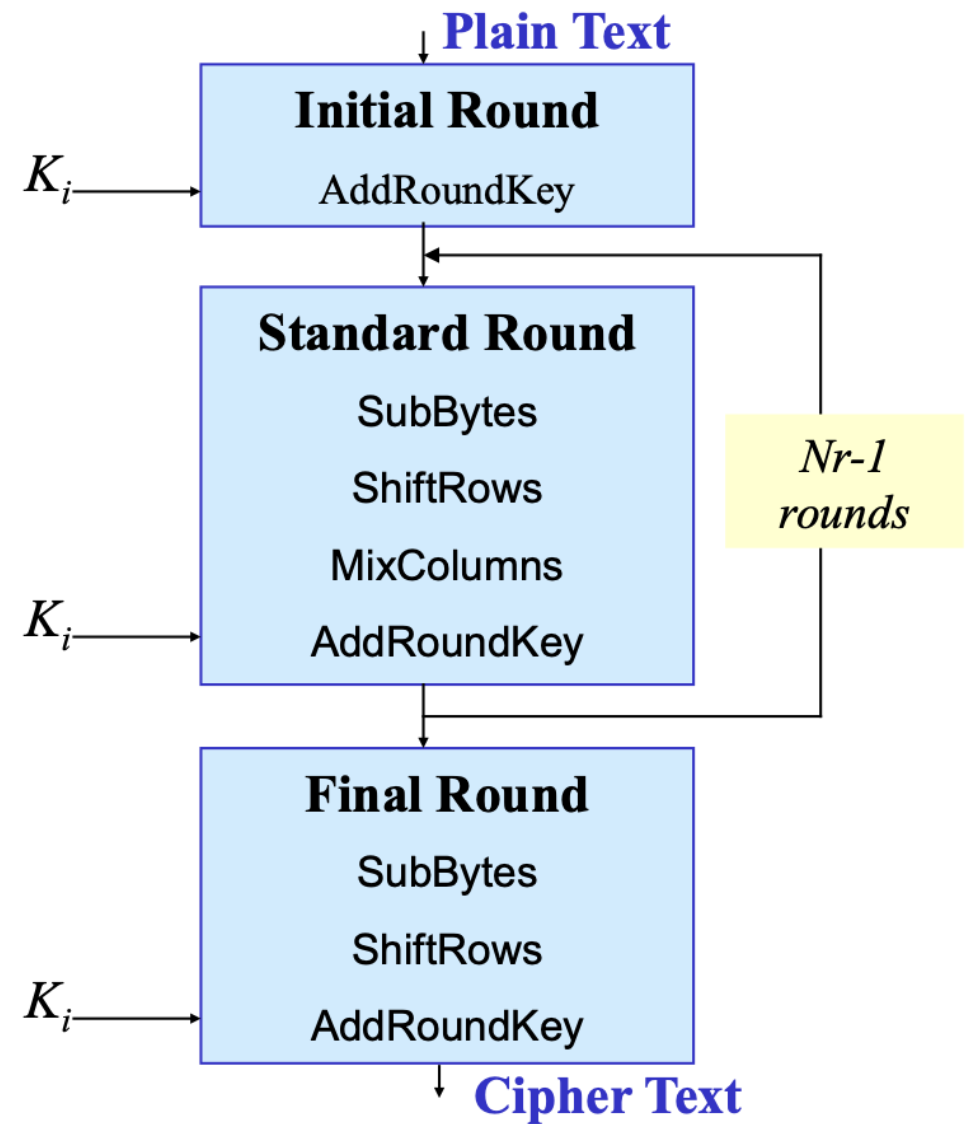
\includegraphics[width=0.3\textwidth]{img/AES.png}
    \caption{Overview of rounds in AES encryption}
    \label{fig:aes}
\end{figure}

\textbf{AddRoundKey}
This operatation takes the state matrix and XORs it, byte by byte, with the round key matrix. The inverse of this operation is clearly the same operation. \\

\textbf{SubBytes}\\
The SubBytes operation in the AES algorithm is a simple substitution step that replaces each byte in the state with another byte using a fixed substitution box (S-box).
Criteria for S-Box:
\begin{itemize}
    \item S-box must be resistant against linear and differential cryptanalysis
    \item S-box must be simple
    \item S-box must be invertible
\end{itemize}

\textbf{ShiftRows}
The ShiftRows operation performs a cyclic shit on the state matrix. Each row is shifted by a different offset (row 1 with 0, row 2 with 1, etc.) \\

\textbf{MixColumns}
This operation ensures that the rows in the state matrix ``interact" with each other over a number of rounds; combined with the ShiftRows operation it ensures each byte of the output state depends on each byte of the input state.
Each column in the state $[ a_0, a_1, a_2, a_3]$ is considered one at a time to create a new column $[b_0, b_1, b_2, b_3]$. This is done by taking the polynomial
\[ a(X) = a_0 + a_1 \cdot X + a_2 \cdot X^2 + a_3 \cdot X^3 \]
and multiplying it by the polynomial $c(X)$ that was chosen for AES to maximize diffusion.
\[ 
c(X) = \texttt{0x02} + \texttt{0x01} \cdot X + \texttt{0x01}  \cdot X^2 + \texttt{0x03}  \cdot X^3
\]

Then the modulo is taken with the invertible polynomial $M(X)$ to ensure invertibility of the MixColumns operation.

\[ M(X) = X^4 + 1 \]

This can be represented by a multiplication matrix (see book and slides) that is invertible in $\mathbb{F}_{2^8}$.


\begin{figure}[h!]
    \centering
    \begin{subfigure}[t]{0.45\textwidth}
        \centering
        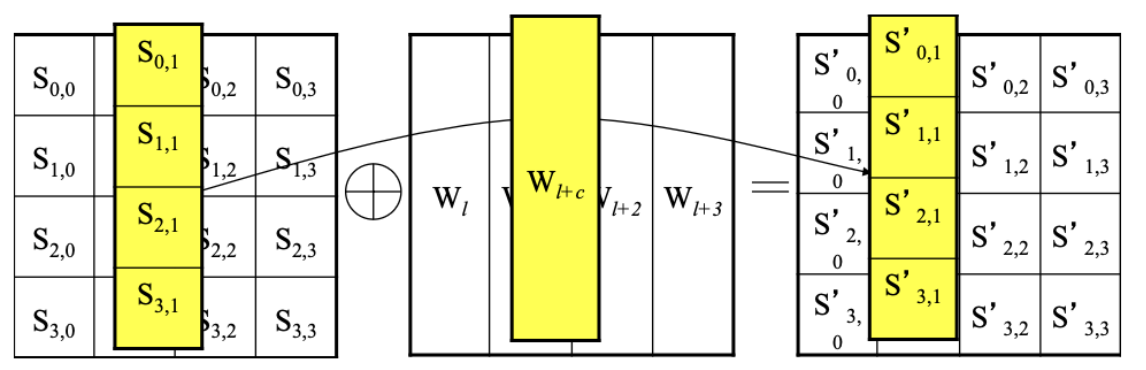
\includegraphics[width=\textwidth]{img/addroundkey.png}
        \caption{Add Round Key}
    \end{subfigure}
    \hfill
    \begin{subfigure}[t]{0.45\textwidth}
        \centering
        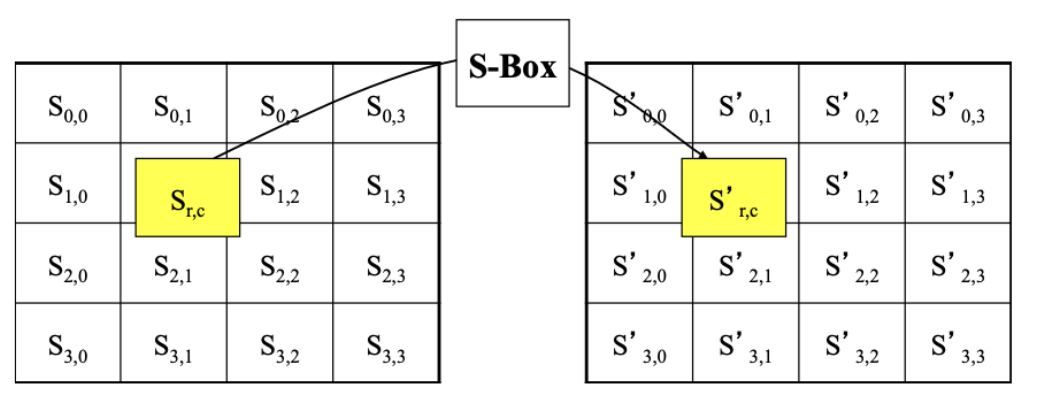
\includegraphics[width=\textwidth]{img/subbytes.png}
        \caption{Sub Bytes}
    \end{subfigure}
    \vfill
    \begin{subfigure}[t]{0.45\textwidth}
        \centering
        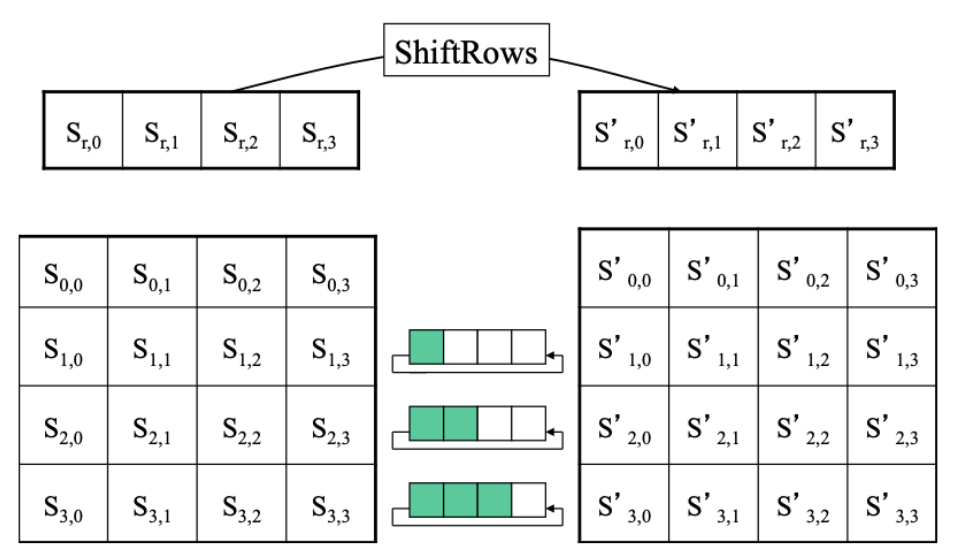
\includegraphics[width=\textwidth]{img/shiftrows.png}
        \caption{Shift Rows}
    \end{subfigure}
    \hfill
    \begin{subfigure}[t]{0.45\textwidth}
        \centering
        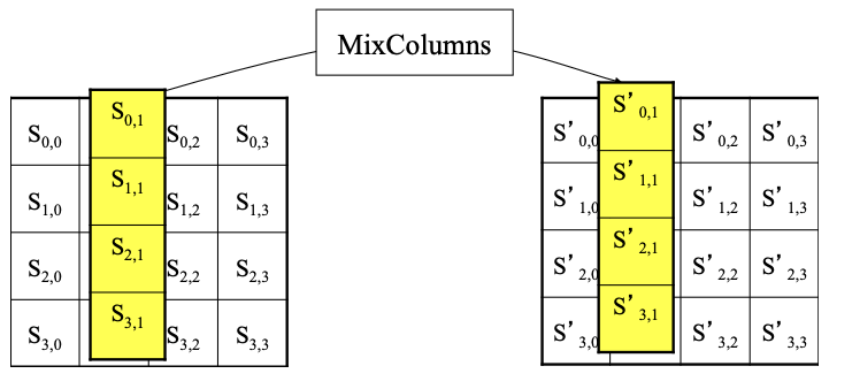
\includegraphics[width=\textwidth]{img/mixcolumns.png}
        \caption{Mix Columns}
    \end{subfigure}
    \caption{AES Operations visualized}
    \label{fig:aes-operations}
\end{figure}

\subsubsection{Key Scheduling}
The AES key schedule generates a series of round keys from the initial secret key. These round keys are used in each round of AES encryption or decryption. Here, we focus on AES with 128-bit blocks. \\


The main key is 128 bits long, and we need to produce 11 round keys $K_0,...,K_{11}$ all of which consist of four 32-bit words, each word corresponding to a column of the matrix K as described above.
The secret key is split into 4-byte words: for AES-128, the key has 4 words \( W_0, W_1, W_2, W_3 \). 
AES requires a separate \textbf{round key} for each encryption round, here: 10 rounds → 11 round keys (each 16 bytes). The round keys are derived using a process called \textbf{key expansion}:

\begin{itemize}
    \item \textbf{RotWord}:
    \begin{itemize}
        \item Rotate the bytes in a word to the left by one position.
        \item Example: \( [b_0, b_1, b_2, b_3] \rightarrow [b_1, b_2, b_3, b_0] \).
    \end{itemize}
    
    \item \textbf{SubWord}:
    \begin{itemize}
        \item Substitute each byte of the word using the AES S-box (just like in the SubBytes step of AES).
    \end{itemize}
    
    \item \textbf{RC}:
    \begin{itemize}
        \item Add a constant value, called the \textbf{round constant}, to the first byte of the word. This ensures that each round key is different.
    \end{itemize}
\end{itemize}

\Comment{Finish this later, i dont really get it...}

\begin{figure}[h!]
    \centering
    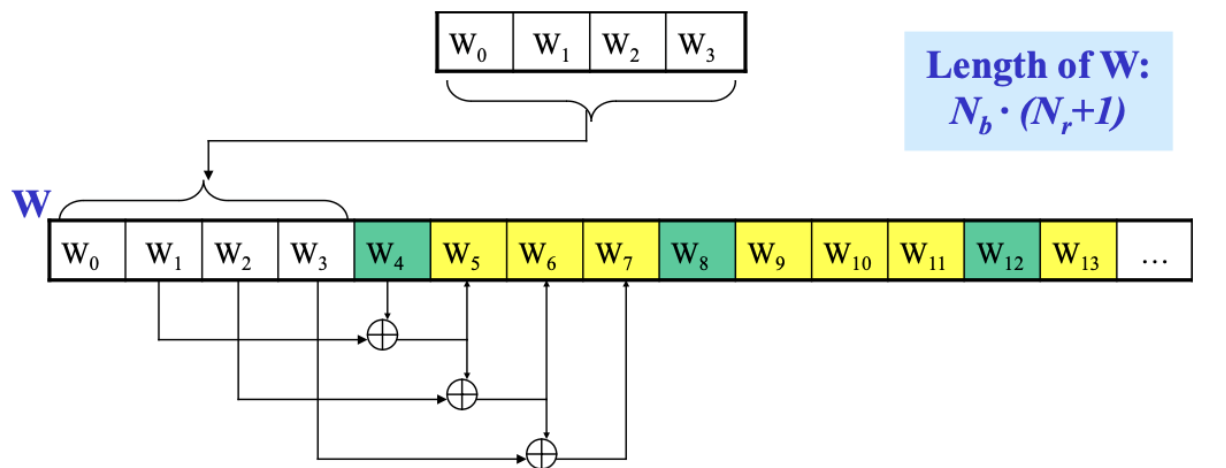
\includegraphics[width=0.5\textwidth]{img/AESkeyschedule.png}
    \caption{AES Key Scheduling}
\end{figure}

\subsubsection{Encryption and Decryption}

\begin{figure}[h!]
    \centering
    \begin{subfigure}[t]{0.40\textwidth}
        \centering
        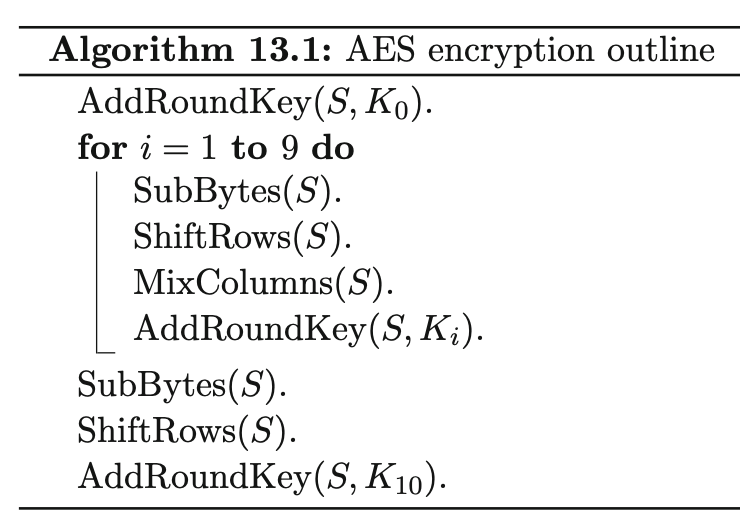
\includegraphics[width=\textwidth]{img/AESencrypt.png}
        \end{subfigure}
        \hfill
        \begin{subfigure}[t]{0.40\textwidth}
            \centering
            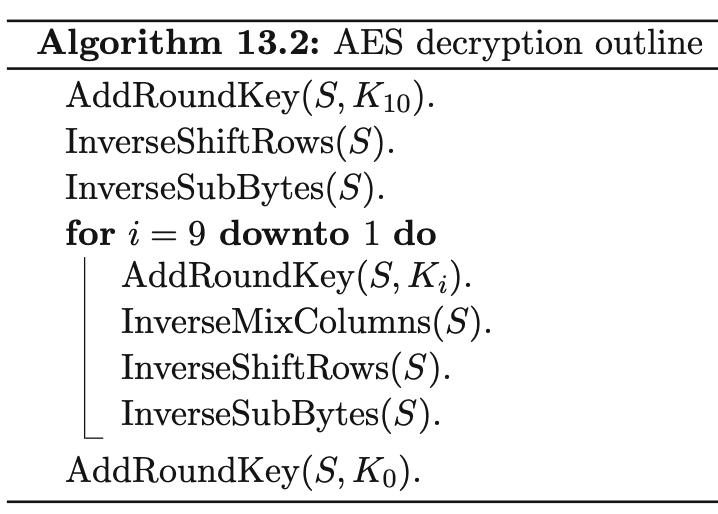
\includegraphics[width=\textwidth]{img/AESdecrypt.png}
        \end{subfigure}
    \caption{Pseudocode for AES Encryption and Decryption}
\end{figure}

\subsection{DES vs. AES}
\begin{table}[h!]
    \centering
    \begin{tabular}{|>{\raggedright\arraybackslash}m{4cm}|>{\raggedright\arraybackslash}m{6cm}|>{\raggedright\arraybackslash}m{6cm}|}
    \hline
    \textbf{Feature} & \textbf{DES} & \textbf{AES} \\
    \hline
    Performance & Fast in hardware, slower in software & Fast in hardware and software \\
    \hline
    Key Length & One key length (not expandable) & Multiple key lengths (expandable in the future) \\
    \hline
    Block Length & One block length (not expandable) & Multiple block lengths \\
    \hline
    Number of Iterations & Many iterations (Feistel structure) & Relatively small amount of iterations \\
    \hline
    \end{tabular}
    \caption{Comparison of DES and AES}
\end{table}



\subsection{Modes of Operation}
Originally, 4 standard modes:
\begin{itemize}
    \item ECB (Electronic Codebook)
    \item CBC (Cipher Block Chaining)
    \item CFB (Cipher Feedback)
    \item OFB (Output Feedback)
\end{itemize}

Over the years, many more: CTR (Counter Mode)

\subsubsection{Electronic Codebook (ECB)}

\subsubsection{Cipher Block Chaining (CBC)}

\subsubsection{Cipher Feedback (CFB)}

\subsubsection{Output Feedback (OFB)}

\subsubsection{Counter Mode (CTR)}

\subsubsection{Security: how to achieve CCA?}